\documentclass[letterpaper]{scrartcl}
\usepackage{tabularx}
\usepackage[none]{hyphenat}
\usepackage[utf8x]{inputenc}
\usepackage{lmodern,textcomp}
\usepackage{enumitem}
\usepackage[final]{pdfpages}
\usepackage{ltablex}
\usepackage[english]{babel}
\usepackage{blindtext}
\usepackage{microtype}
\usepackage[hidelinks]{hyperref}
\usepackage{hanging}
\usepackage[paperheight=279.4mm,paperwidth=210mm,bottom=10em]{geometry}
\usepackage{fancyhdr}
\setlength{\parskip}{1em}

\pagestyle{fancy}
\fancyhf{}
\fancyhead[LE,LO]{Anthony Kevins}
\fancyhead[RE,RO]{Documentation of Knowledge Dissemination}
\fancyfoot[CE,CO]{\leftmark}
\fancyfoot[CE,CO]{\thepage}
\setlength\parindent{0pt}
\setlist[itemize]{leftmargin=*}

\begin{document}

  I am committed to ensuring that my research output reaches the broadest possible audience, including the general public, experts, and policy makers. In order to help demonstrate this commitment, this document provides several examples of the knowledge dissemination activities I have undertaken.

  The following pages thus include copies of:\\[-4ex]

  \begin{itemize}
    \item A newspaper article referencing some of my research with Stuart Soroka. The article was published in the Globe \& Mail (Canada's newspaper of record) after the journalist reached out to us. \\[-4ex]
    \item A presentation that I made at the Municipality of Aarhus's Department of Health and Care (Sundhed og Omsorg, Aarhus Kommune). I was invited to give an hour-long talk on eldercare and healthcare in the US in preparation for a consultation the Department was about to undertake in California. \\[-4ex]
    \item A blog post that I wrote with Carsten Jensen on the LSE's British Politics \& Policy Blog. The entry was written for a general audience and designed to communicate the main findings from an article we had just published.
  \end{itemize}

  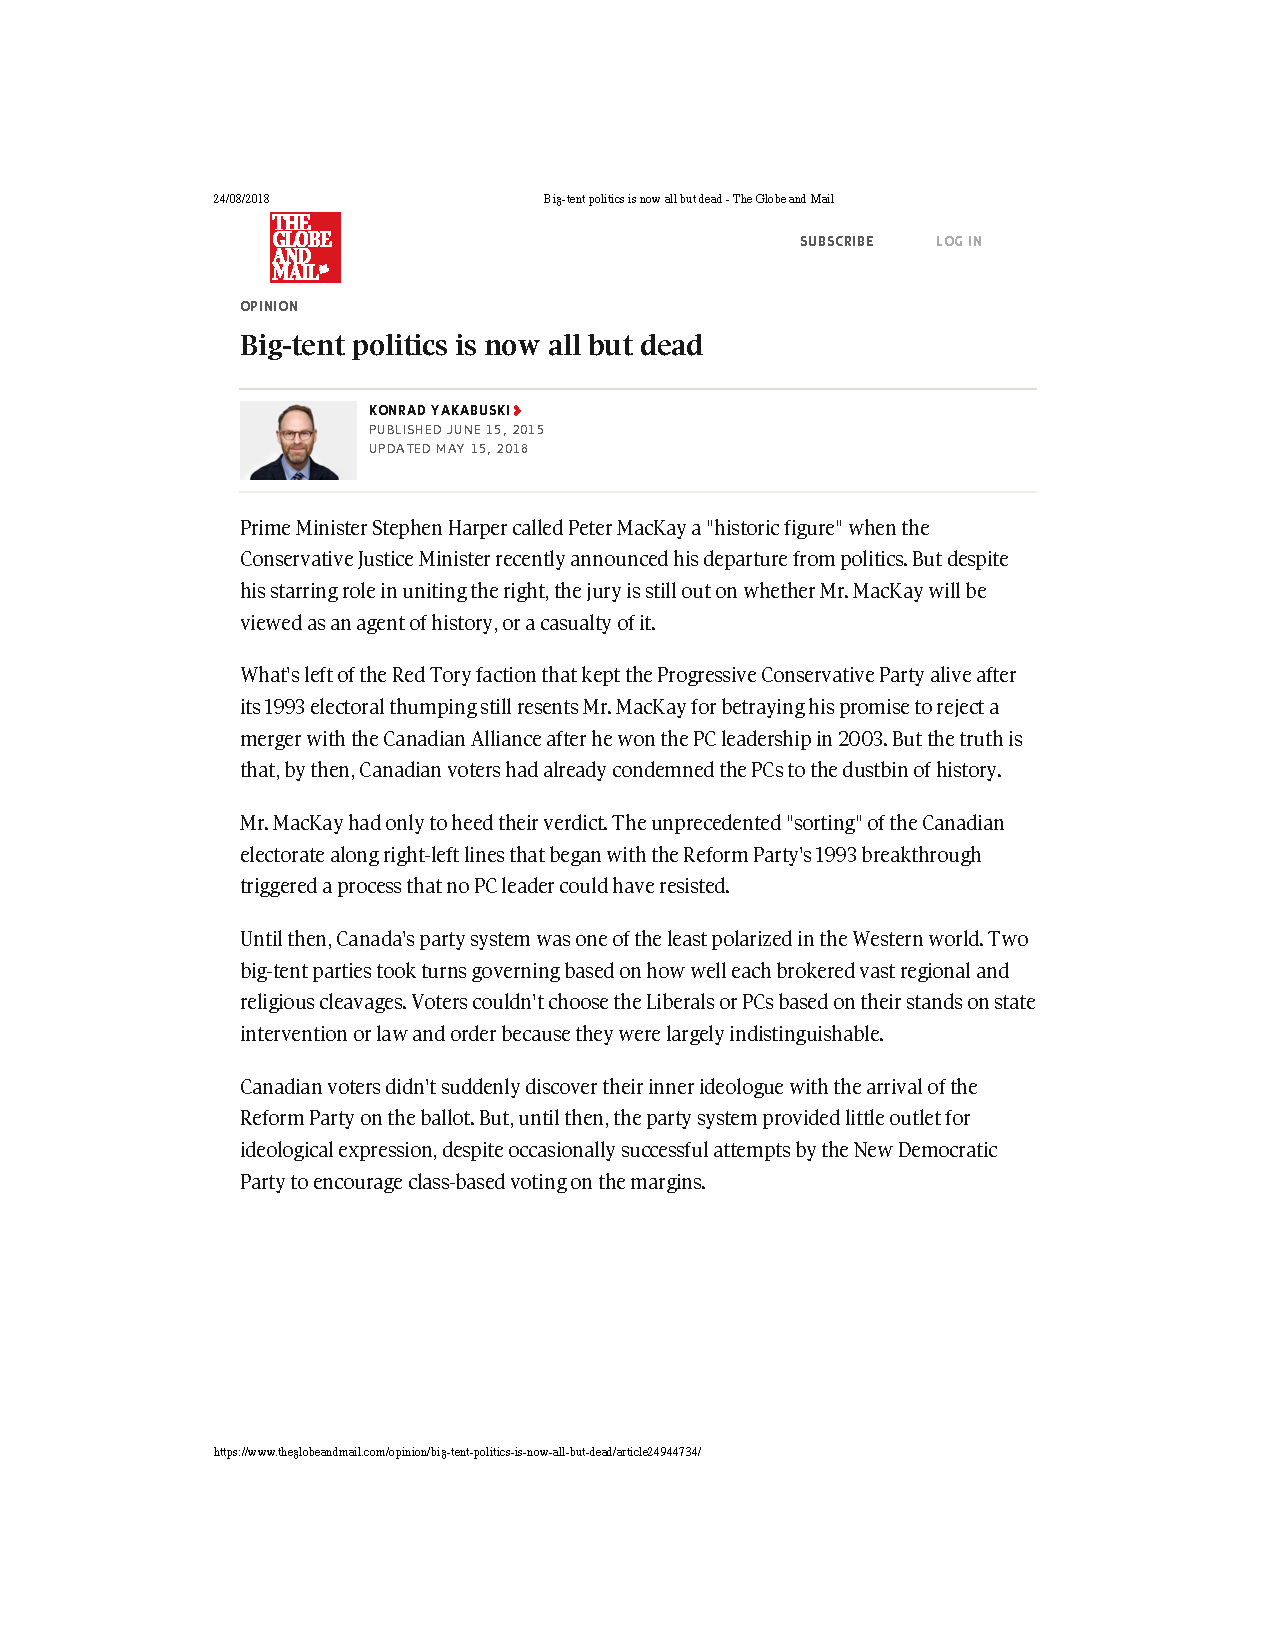
\includepdf[pages=-,pagecommand={},]{Appendix.pdf}


\end{document}
